\documentclass[border=4pt]{standalone}
% Preámbulo común de las figuras. Cada figura es un documento standalone
% que se compila a SVG con scripts/build_figures.sh
\usepackage[utf8]{inputenc}
\usepackage{amsmath}
\usepackage{tikz}
\usepackage[american, siunitx]{circuitikz}
\usetikzlibrary{arrows.meta,calc,decorations.pathmorphing,patterns}
\tikzset{
  >={Stealth[length=2.2mm]},
  eje/.style={->, thin},
  hilo/.style={thick},
}
% Paleta común: tonos medios legibles sobre fondo claro
\definecolor{azul}{RGB}{31,94,168}
\definecolor{rojo}{RGB}{192,57,43}
\definecolor{verde}{RGB}{39,128,73}
\definecolor{naranja}{RGB}{211,120,30}
\definecolor{morado}{RGB}{125,60,152}

\begin{document}
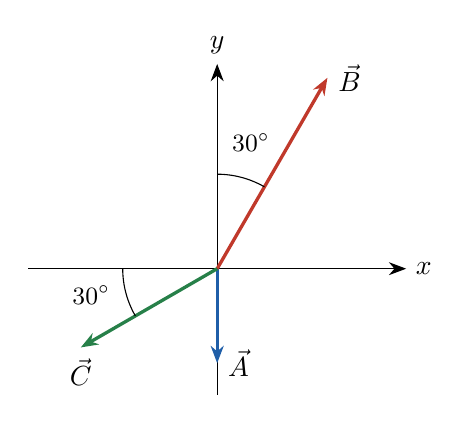
\begin{tikzpicture}[scale=0.2]
  \draw[eje] (-12,0) -- (12,0) node[right]{$x$};
  \draw[eje] (0,-8) -- (0,13) node[above]{$y$};
  \draw[->, very thick, azul] (0,0) -- (0,-6) node[right, text=black]{$\vec A$};
  \draw[->, very thick, rojo] (0,0) -- (60:14) node[right, text=black]{$\vec B$};
  \draw (0,6) arc (90:60:6); \node[font=\small] at (75:8.3) {$30^\circ$};
  \draw[->, very thick, verde] (0,0) -- (210:10) node[below, text=black]{$\vec C$};
  \draw (-6,0) arc (180:210:6); \node[font=\small, anchor=east] at (195:6.4) {$30^\circ$};
\end{tikzpicture}
\end{document}
